\section{Implementazione}
\begin{frame}{Implementazione}
    Per implementare un servizio onion è necessario utilizzare il \textbf{Proxy Onion} per inoltrare le richieste dalla rete Tor al server web, il proxy gestisce la generazione delle chiavi, dell'indirizzo e la definizione e connessione con gli \textbf{introduction points}, oltre alla generazione del descriptor e la sua pubblicazione nei Directory Servers. \\
    In particolare la nostra implementazione userà \textbf{Onion V3} (dato che Onion V2 è stato deprecato) con alcune migliorie tra cui la maggior sicurezza degli indirizzi. \\
    Useremo un server \textbf{Linux EC2} di AWS per ospitare il proxy onion e un \textbf{server nginx}.
\end{frame}

\begin{frame}
    Nel sistema è necessario installare il pacchetto nginx (web server) e dopo una serie di configurazioni dei repository possiamo installare tor. 
    \newline
    Configuriamo il file di configurazione torrc con \lstinline{HiddenServiceDir /var/lib/tor/hidden_service} (per indicare la directory dove verranno salvate le chiavi) e \lstinline{HiddenServicePort 80 unix:/var/run/website.sock} (per indicare il tipo e il modo di connessione con il web server). \\
    In questa implementazione abbiamo usato un tool (mkp224o) per generare la coppia chiave privata e pubblica che risulti in un indirizzo onion personalizzato.
\end{frame}

\begin{frame}
    \begin{figure}
        \centering
        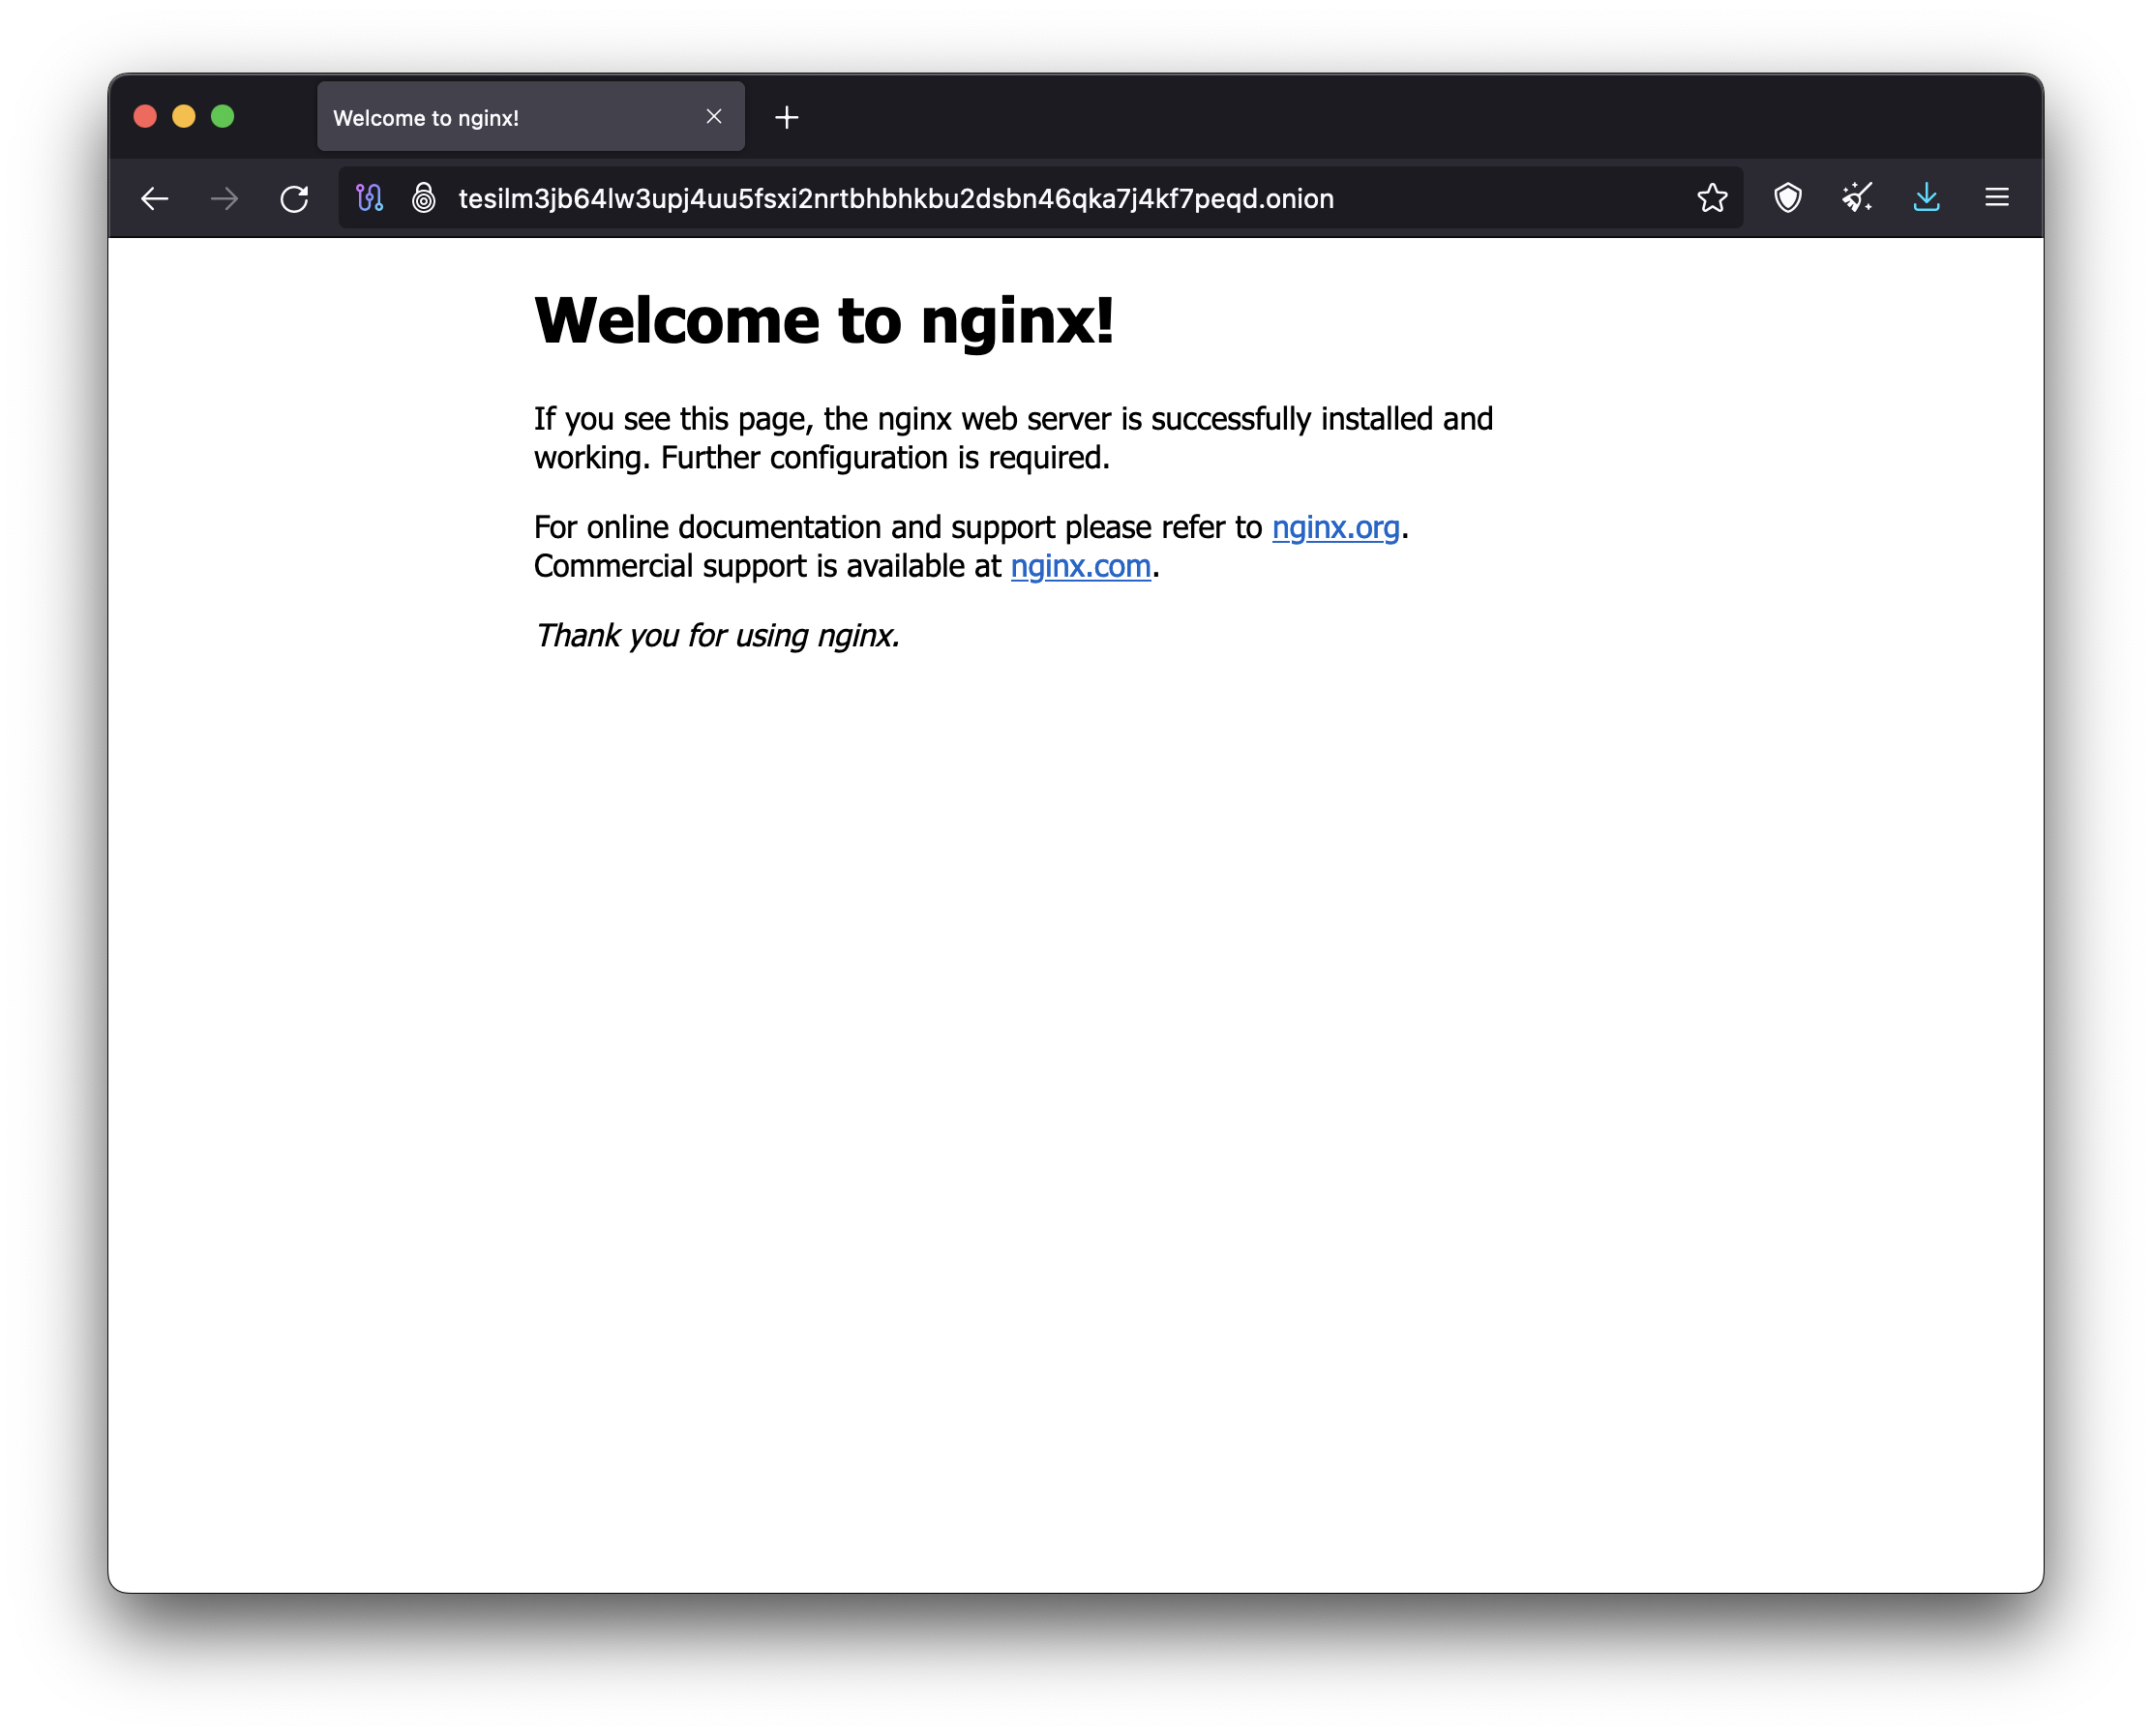
\includegraphics[width=\textwidth]{connectionCustomAddress.png}
    \end{figure}
\end{frame}

\subsection{Pubblicizzare il servizio}
\begin{frame}{Pubblicizzare il servizio}
    Nel lavoro di tesi abbiamo mostrato 2 principali sistemi per pubblicizzare il servizio:
    \begin{itemize}
        \item Pubblicizzazione su altri siti o motori di ricerca, come \textbf{notEvil} o \textbf{OnionDir}
        \item \textbf{Header Tag}, è possibile inserire un tag all'interno di un sito web che quando aperto con Tor consente di reindirizzare l'utente al relativo sito onion, in maniera automatica o tramite il tasto in alto a sinistra.
    \end{itemize}
    \lstinline{<meta http-equiv="onion-location" content="http://tesilm3jb64lw3upj4uu5fsxi2nrtbhbhkbu2dsbn46qka7j4 kf7peqd.onion" />}
    % The space is important to make the line break correctly
\end{frame}

\begin{frame}
    \begin{figure}
        \centering
        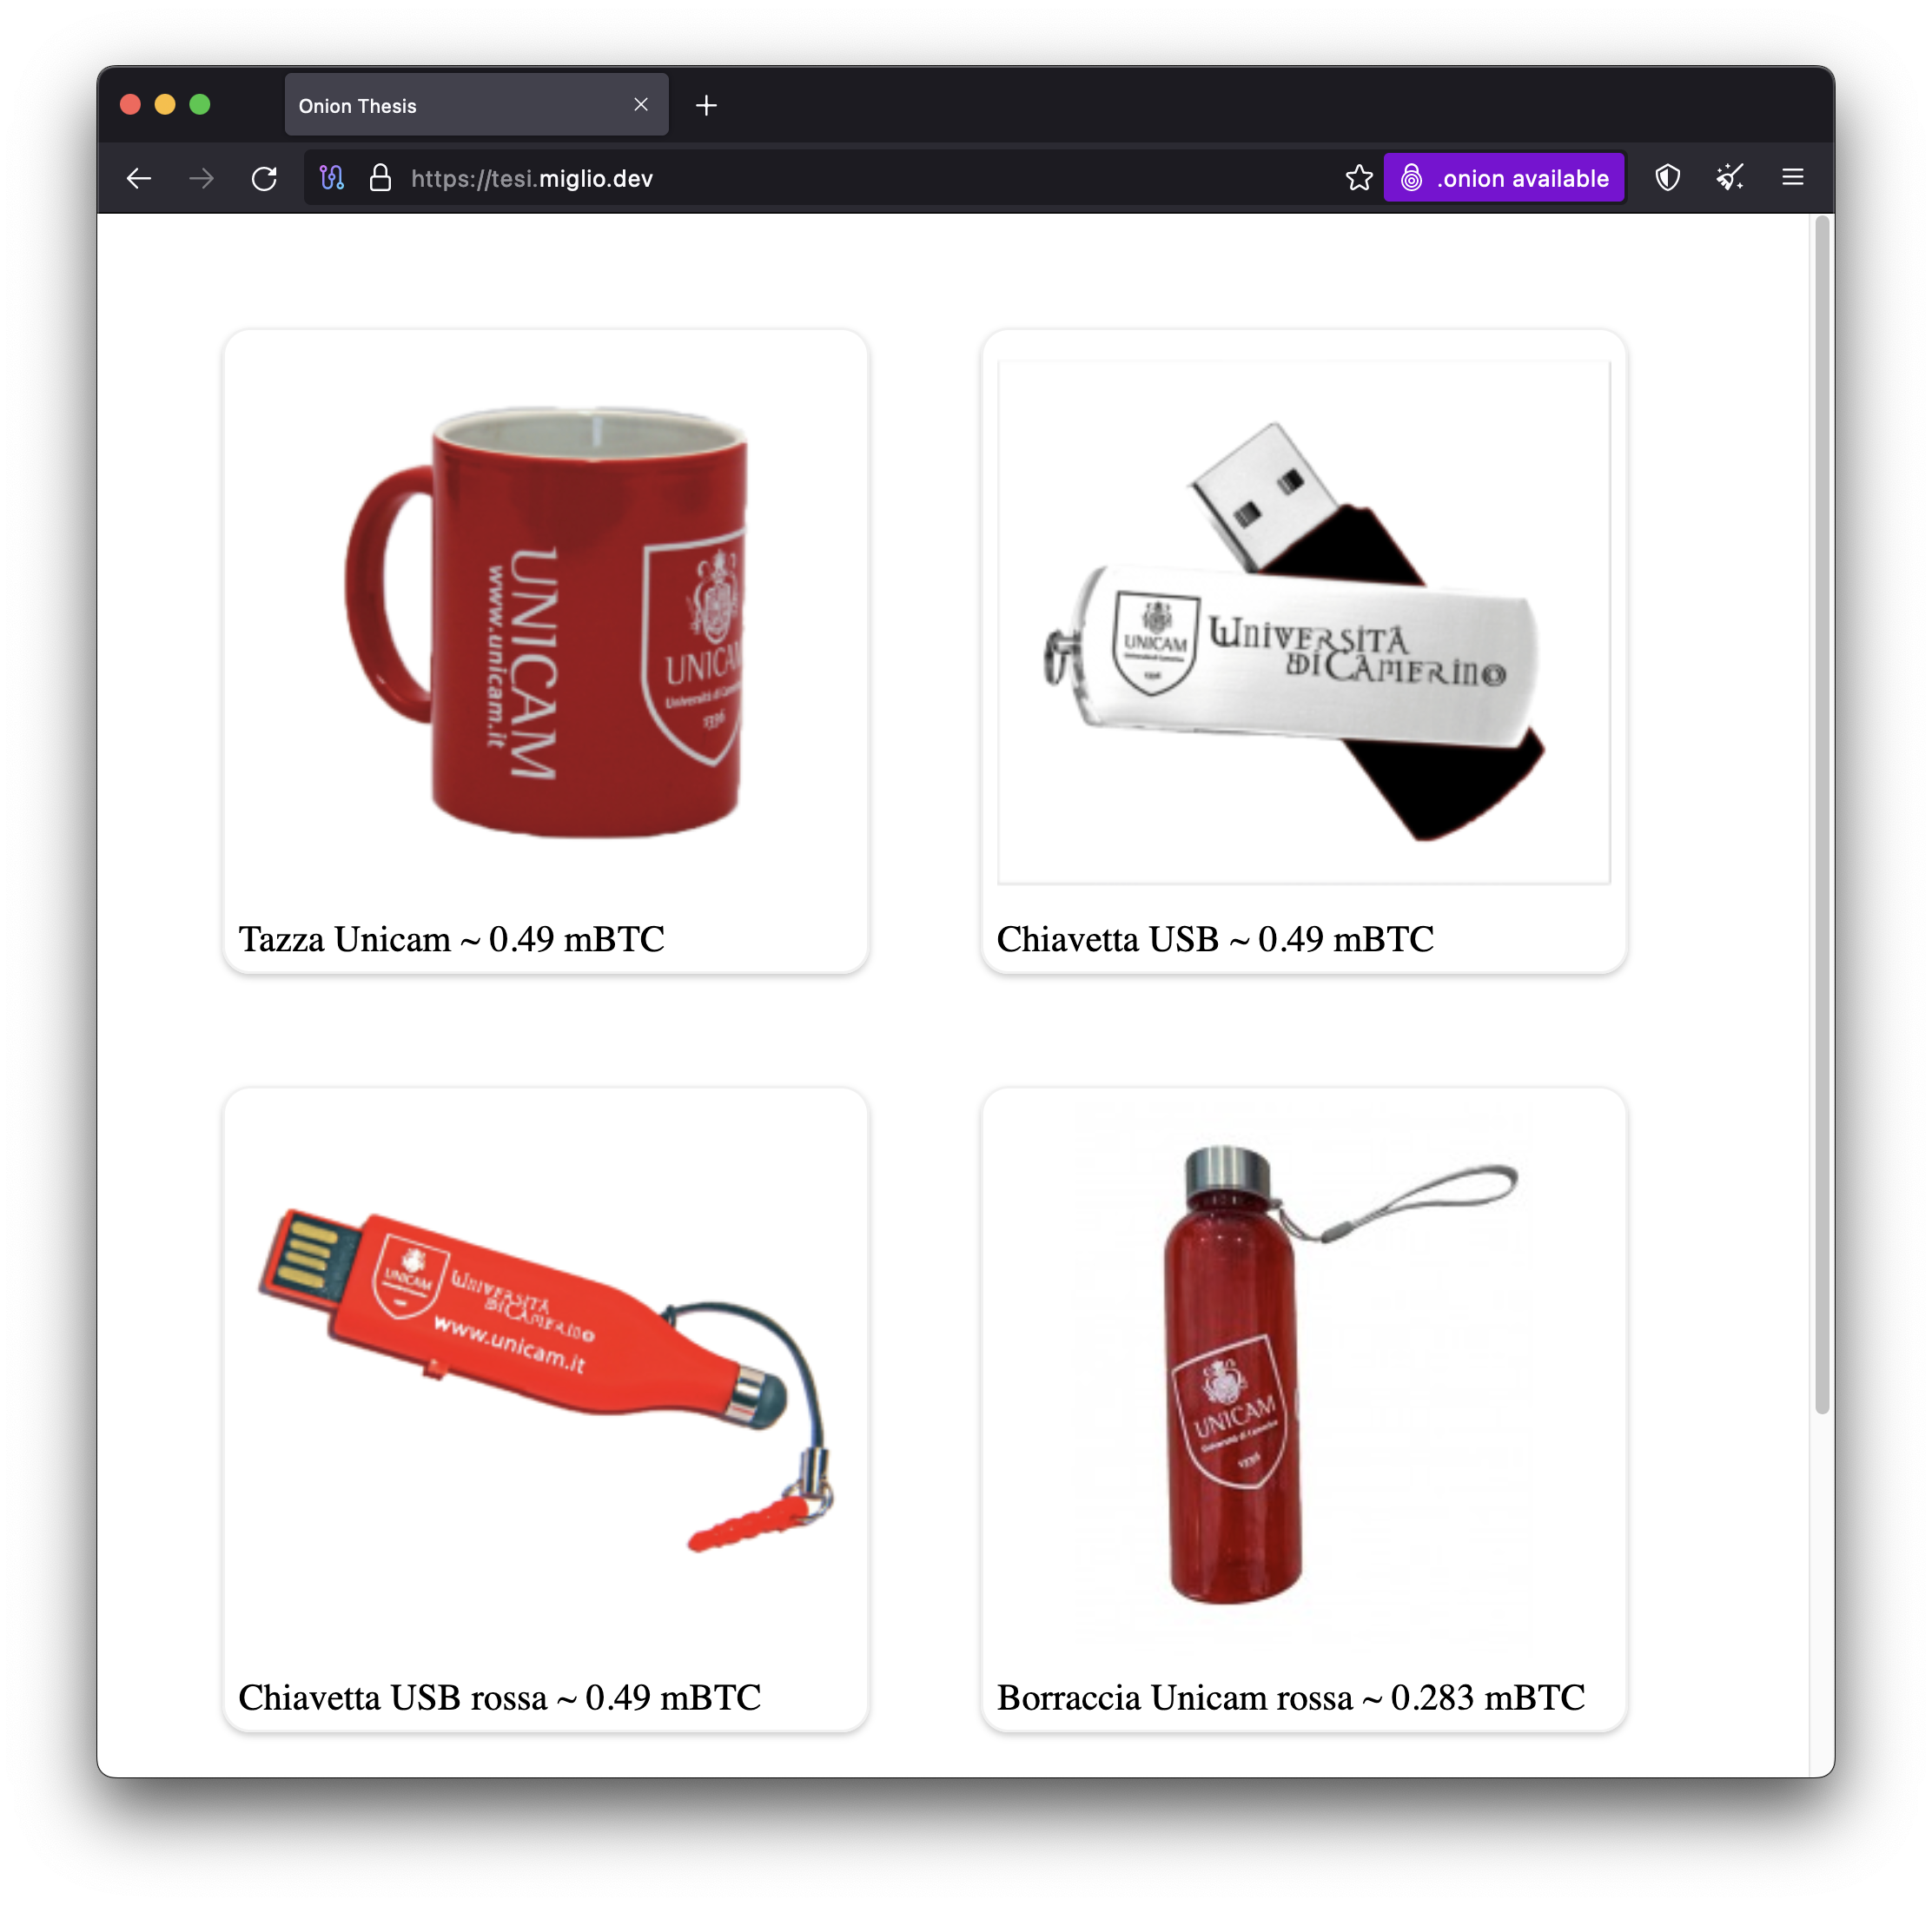
\includegraphics[width=0.8\textwidth]{ClearWebPage}
    \end{figure}
\end{frame}

